\documentclass[11pt, a4paper]{report}
\usepackage[utf8]{inputenc}
\usepackage{pgfplots}

\usepackage[top=2cm, bottom=2.3cm, left=2cm, right=2cm]{geometry}

\title{Graficos das geracoes do NSGA2}
\author{Douglas Nunes de Oliveira}
\date{November 2021}


\begin{document}
    \begin{center}
        \textbf{Utilizando o NSGA2 para o problema de Schaffer modificado.}
        
        \textbf{Gráficos do espaço dos objetivos nas gerações ``1, 10, 50, 100 e 1000''}
        
        
    \end{center}
    

    \begin{center}
    \textbf{Geração 1}
\end{center}

\begin{figure}[h]
    \centering
    \label{fig:geracao01}
    
    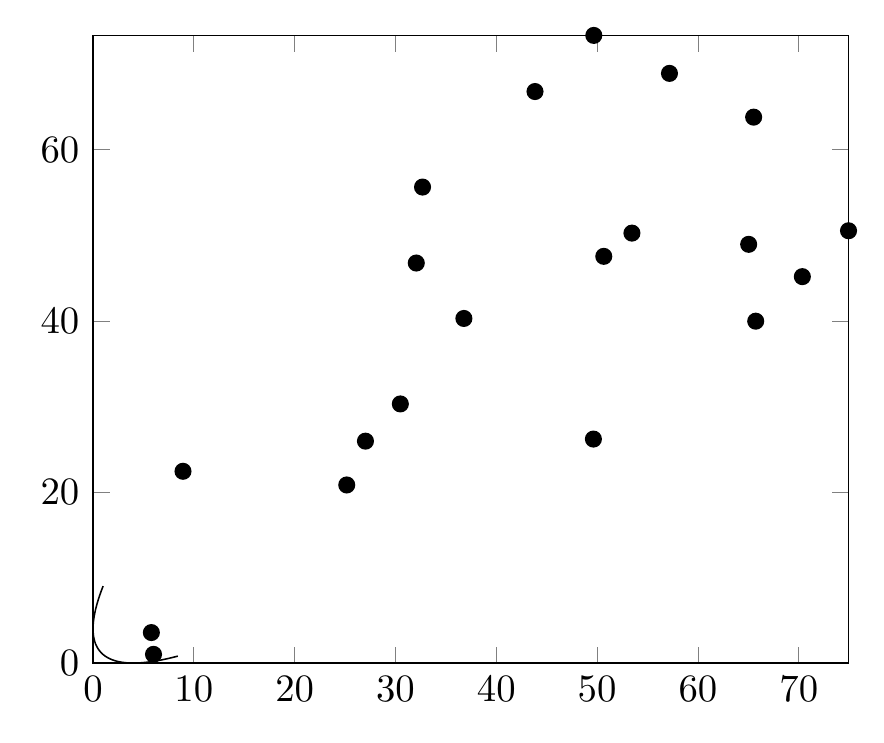
\begin{tikzpicture}[scale=1.4]
        \begin{axis}[enlargelimits=false]
            \addplot [] coordinates {
                (1.000000,9.000000) (0.810000,8.410000) (0.640000,7.840000) (0.490000,7.290000) (0.360000,6.760000) (0.250000,6.250000) (0.160000,5.760000) (0.090000,5.290000) (0.040000,4.840000) (0.010000,4.410000) (0.000000,4.000000) (0.010000,3.610000) (0.040000,3.240000) (0.090000,2.890000) (0.160000,2.560000) (0.250000,2.250000) (0.360000,1.960000) (0.490000,1.690000) (0.640000,1.440000) (0.810000,1.210000) (1.000000,1.000000) (1.210000,0.810000) (1.440000,0.640000) (1.690000,0.490000) (1.960000,0.360000) (2.250000,0.250000) (2.560000,0.160000) (2.890000,0.090000) (3.240000,0.040000) (3.610000,0.010000) (4.000000,0.000000) (4.410000,0.010000) (4.840000,0.040000) (5.290000,0.090000) (5.760000,0.160000) (6.250000,0.250000) (6.760000,0.360000) (7.290000,0.490000) (7.840000,0.640000) (8.410000,0.810000) 
            };
            
            \addplot [only marks] coordinates {
                (5.787295,3.564607) (6.000384,1.019951) (8.924366,22.422057) (25.165956,20.822240) (27.021558,25.945465) (49.632034,26.187191) (30.481920,30.297171) (32.062254,46.769869) (36.784962,40.289392) (65.730368,39.971138) (32.684037,55.650321) (50.659824,47.551207) (70.355101,45.178097) (43.838685,66.820797) (53.453039,50.267766) (65.031091,48.956057) (74.934630,50.543697) (49.671026,73.381278) (65.525429,63.825250) (57.175333,68.942821) 
            };
        \end{axis}
    \end{tikzpicture}
    
\end{figure}

    \hrulefill
    \begin{center}
    \textbf{Geração 10}
\end{center}

\begin{figure}[h]
    \centering
    \label{fig:geracaoXX}
    
    \begin{tikzpicture}[scale=1.4]
        \begin{axis}[enlargelimits=false]
            \addplot [] coordinates {
                (0.000000,4.000000) (0.010000,3.610000) (0.040000,3.240000) (0.090000,2.890000) (0.160000,2.560000) (0.250000,2.250000) (0.360000,1.960000) (0.490000,1.690000) (0.640000,1.440000) (0.810000,1.210000) (1.000000,1.000000) (1.210000,0.810000) (1.440000,0.640000) (1.690000,0.490000) (1.960000,0.360000) (2.250000,0.250000) (2.560000,0.160000) (2.890000,0.090000) (3.240000,0.040000) (3.610000,0.010000) (4.000000,0.000000) 
            };
            
            \addplot [only marks] coordinates {
                (9.765582,16.939883)(9.924204,17.003386)(10.091199,17.110039)(10.211898,17.205926)(10.337007,17.555696)(12.514860,17.518859)(13.126414,18.337417)(17.804570,20.690929)(70.410450,56.563290)(71.896435,90.028819)(72.099991,90.135653)(72.732258,90.743713)(72.980565,91.249132)(73.640637,91.289447)(73.857270,91.995217)(75.358388,92.246202)(75.811555,94.296171)(76.248114,94.129894)(76.362091,94.174254)(76.250749,94.632550) 
            };
        \end{axis}
    \end{tikzpicture}
\end{figure}

    \newpage

    \begin{center}
    \textbf{Geração 50}
\end{center}

\begin{figure}[h]
    \centering
    \label{fig:geracaoXX}
    
    \begin{tikzpicture}[scale=1.4]
        \begin{axis}[enlargelimits=false]
            \addplot [] coordinates {
                (0.000000,4.000000) (0.010000,3.610000) (0.040000,3.240000) (0.090000,2.890000) (0.160000,2.560000) (0.250000,2.250000) (0.360000,1.960000) (0.490000,1.690000) (0.640000,1.440000) (0.810000,1.210000) (1.000000,1.000000) (1.210000,0.810000) (1.440000,0.640000) (1.690000,0.490000) (1.960000,0.360000) (2.250000,0.250000) (2.560000,0.160000) (2.890000,0.090000) (3.240000,0.040000) (3.610000,0.010000) (4.000000,0.000000) 
            };
            
            \addplot [only marks] coordinates {
                (7.079039,9.893604)(6.998996,10.667901)(7.153247,10.267265)(7.675170,10.023482)(7.176644,10.167450)(7.684816,10.057420)(7.337534,10.589789)(7.258915,11.093974)(7.387049,10.466614)(7.385134,10.873843)(7.421006,10.594347)(7.413217,11.198653)(7.536725,10.792519)(7.722630,10.658570)(7.437473,10.984634)(7.596418,10.718251)(7.577853,11.008782)(7.721938,10.867479)(8.215063,10.807069)(8.124915,10.913137)
            };
        \end{axis}
    \end{tikzpicture}
\end{figure}
    \hrulefill
    \begin{center}
    \textbf{Geração 100}
\end{center}

\begin{figure}[h]
    \centering
    \label{fig:geracaoXX}
    
    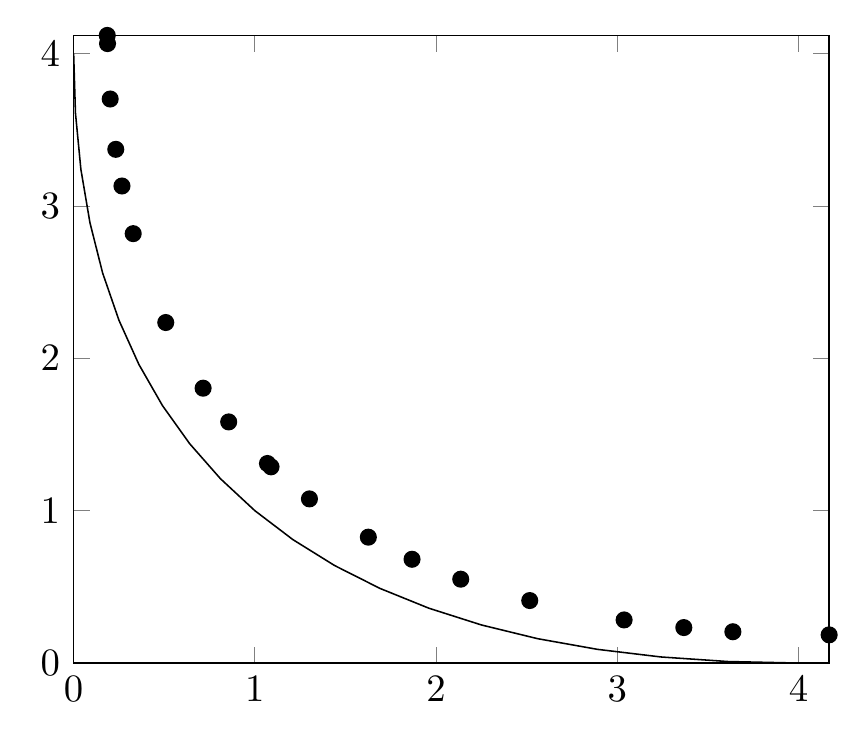
\begin{tikzpicture}[scale=1.4]
        \begin{axis}[enlargelimits=false]
            \addplot [] coordinates {
                (0.000000,4.000000) (0.010000,3.610000) (0.040000,3.240000) (0.090000,2.890000) (0.160000,2.560000) (0.250000,2.250000) (0.360000,1.960000) (0.490000,1.690000) (0.640000,1.440000) (0.810000,1.210000) (1.000000,1.000000) (1.210000,0.810000) (1.440000,0.640000) (1.690000,0.490000) (1.960000,0.360000) (2.250000,0.250000) (2.560000,0.160000) (2.890000,0.090000) (3.240000,0.040000) (3.610000,0.010000) (4.000000,0.000000) 
            };
            
            \addplot [only marks] coordinates {
                (4.168578,0.185014) (0.185481,4.119608) (0.508235,2.235170) (1.301067,1.077486) (0.714368,1.804074) (0.328600,2.818474) (1.625955,0.826308) (0.855511,1.582758) (1.069318,1.309841) (0.201713,3.702131) (2.516477,0.410313) (1.089113,1.288015) (3.037264,0.283012) (0.186988,4.065829) (0.232462,3.371838) (1.867110,0.681172) (3.366609,0.232987) (2.135822,0.550495) (3.637344,0.205522) (0.266636,3.131241) 
 
            };
        \end{axis}
    \end{tikzpicture}
\end{figure}
    
    \newpage
    \begin{center}
    \textbf{Geração 1000}
\end{center}

\begin{figure}[h]
    \centering
    \label{fig:geracaoXX}
    
    \begin{tikzpicture}[scale=1.4]
        \begin{axis}[enlargelimits=false]
            \addplot [] coordinates {
                (0.000000,4.000000) (0.010000,3.610000) (0.040000,3.240000) (0.090000,2.890000) (0.160000,2.560000) (0.250000,2.250000) (0.360000,1.960000) (0.490000,1.690000) (0.640000,1.440000) (0.810000,1.210000) (1.000000,1.000000) (1.210000,0.810000) (1.440000,0.640000) (1.690000,0.490000) (1.960000,0.360000) (2.250000,0.250000) (2.560000,0.160000) (2.890000,0.090000) (3.240000,0.040000) (3.610000,0.010000) (4.000000,0.000000) 
            };
            
            \addplot [only marks] coordinates {
                (3.999653,0.000005) (0.000005,4.000680) (2.671273,0.133667) (0.377116,1.920741) (0.536675,1.606364) (2.176495,0.275322) (3.535918,0.014308) (0.098021,2.845721) (0.992605,1.007433) (2.947273,0.080229) (0.686426,1.372405) (1.599510,0.540648) (0.022028,3.428415) (0.287709,2.142187) (1.238691,0.786840) (1.839518,0.414372) (2.101884,0.302740) (0.167266,2.531363) (3.902097,0.000611) (0.200691,2.408770) 
 
            };
        \end{axis}
    \end{tikzpicture}
\end{figure}
    \hrulefill

\end{document}
